
Neste capítulo serão abordadas as técnicas anteriormente mencionadas, que são o foco deste trabalho, PLL (Phase-Locked Loop), análise de prony, ADALINE e RLS (Recursive Least Mean Squares), bem como as convencionais DFT e STFT. É importante ressaltar que esta será apenas uma abordagem superficial, não entrando, portanto, com profundidade nos assuntos tratados.

\section{Análise espectral}
Análise espectral considera o problema de encontrar a energia de um sinal, finito, distribuída em função de frequência, o que pode ser feito com métodos paramétricos ou não paramétricos. Métodos paramétricos assumem conhecimento do modelo com o qual se gerou o sinal em análise. Por exemplo, em alguns capítulos, como o de análise de Prony, é assumido que o sinal é composto unicamente por un número conhecido de exponenciais complexas amortecidas. Para solucionar um problema de estimação paramétrica, o que se deve fazer é encontrar os parâmetros supostos. Por outro lado, métodos não paramétricos se baseiam unicamente em transformações do domínio temporal para o domínio da frequência, utilizando filtros que nos dão a energia do sinal contida em uma determinada faixa do espectro, caso da DFT. Quando temos uma boa estimação de nosso modelo, os métodos paramétricos tendem a dar melhores resultados, enquanto que quando pouco se sabe sobre o sinal analisado, ou se o mesmo não está bem modelado, os não paramétricos podem ser a melhor opção.

\indent Algumas vezes é conveniente tratar os sinais de maneira determinística, e o será feito neste trabalho, entretanto, como abordagem mais geral, se pode tratá-los com enfoque probabilístico, isto é: admitir que não se pode de maneira alguma prever os valores assumidos por um sinal ao longo do tempo, mas se pode estimar suas características por meios estatísticos.
\indent É de se notar também que embora sinais reais sejam o caso mais comum na maioria das aplicações e em nosso caso são praticamente regra, não necessariamente o tratamento de sinais complexos é muito mais complicado. Apenas por uma questão de praticidade e para deixar o trabalho mais conciso, não serão demonstrados os teoremas utilizados para entradas complexas quando não for necessário.\cite{stoica2005spectral}

\section{Densidade espectral de energia de um sinal determinístico}
Seja $y_c(t)$ um sinal contínuo no tempo e $y[n], \; n=0, \pm 1, \pm 2,...$  um sinal discreto tal que $y[n]=y_c(nT_s)$. Considerando que $y[n]$ tem energia finita. Pode-se dizer então que a DTFT de $y$ está definida como:

\begin{equation}
Y(w)=\sum_{n=-\infty}^{+\infty}y[n]e^{-jwn}
\label{eq:DTFT}
\end{equation}

Onde $w$ é denominada frequência angular medido em radianos/segundo, e pode ser relacionada com seu valor físico da seguinte maneira $\bar{w}=wT_s$. A densidade espectral de energia do sinal $y(t)$ pode ser dada então por:
\begin{equation}
S(w)=|Y(w)|^2
\end{equation}

Pode-se interpretar este resultado de algumas formas, mas uma bem simples é lembrar que a DTFT de uma cossenoide é igual a soma de duas deltas refletidas no espectro de frequência:

\begin{equation}
\sum_{n=-\infty}^{+\infty}cos(2\pi f \: n)e^{-jwn}= \pi \delta_{w}(2\pi f) + \pi \delta_{w}(-2\pi f) \;\; w \; \in [0,2 \pi]
\end{equation}

Uma relação muito parecida se estabelece no caso de uma senoide. Desta maneira, quando se imagina $yc(t)$ composta unicamente de uma soma de senoides, seu espectro fica muito bem explicitado com a equação \ref{eq:DTFT}.

Uma outra relação importante se dá utilizando a autocorrelação de $y[n]$:

\begin{equation}
\rho_y[k]=\sum_{n=-\infty}^{+\infty}y[n]y^*[n-k]
\end{equation}

\begin{equation*}
\sum_{k=-\infty}^{+\infty}\rho_y[k]e^{-jwk}=\sum_{n=-\infty}^{+\infty}\sum_{k=-\infty}^{+\infty}y[n]y^*[n-k]e^{-jwk}=
\end{equation*}
\begin{equation}
\begin{aligned}
\sum_{n=-\infty}^{+\infty}\sum_{k=-\infty}^{+\infty}y[n]y^*[n-k]e^{-jwn}e^{jw(n-k)}  = \\ \left[\sum_{n=-\infty}^{+\infty}y[n]e^{-jwn} \right]  \left[\sum_{s=-\infty}^{+\infty}y[s]e^{-jws} \right]^* = Y(w)Y(w)^*
\end{aligned}
\end{equation}

Vê-se então que a DTFT da autocorrelação de um sinal é igual sua densidade espectral de energia.

\subsection{Densidade espectral de potência}

A maioria dos sinais com os quais se trabalha não têm um modelo puramente determinístico que os reproduza, não se sabe o valor exato que tomarão no futuro, e tampouco se pode estender seu valor até o infinito, ou analisar infinitas amostras do mesmo. Para os casos reais, é mais conveniente lidar com sequencias aleatórias ao longo do tempo, em que cada realização da sequência tem associada uma distribuição de probabilidade (até o momento de sua ocorrência, quando esta colapsa em algum valor). Para a maioria dos casos, consideraremos os sinais como processos estacionários em sentido amplo \cite{haykin2005adaptive}. Para este trato aleatório, não é regra que nossos sinais tenham energia finita, mas é possível ao invés disso, estimar sua densidade de potência.

\indent Assume-se agora que $y[n]$ é uma sequência de variáveis aleatórias, com o mesmo domínio da sequência anterior, e que $E[y[n]]=0$ para todo $n$. Tendo todas as variáveis aleatórias média nula. A função de correlação de $y[n]$ está definida como:

\begin{equation}
r_y[k]=E[ y[n] \: y[n-k]^*]
\end{equation}

\indent Definimos então a densidade espectral de potência como:

\begin{equation}
\phi (w)=\sum_{k=-\infty}^{+\infty}r_y[k]e^{-jwk}
\end{equation}

\indent Uma segunda definição para a PSD (\textit{Power Spectrum Density}) pode ser dada como a DTFT do sinal com o número amostras tendendo ao infinito da seguinte forma:

\begin{equation}
\phi(w)=\lim_{N\rightarrow \infty}\frac{1}{N}\left|\sum_{k=0}^{N-1}y[k]e^{-jwk}  \right|^2
\end{equation}

\indent Ambas definições são equivalentes. Será exposto mais adiante que uma das formas principais de se calcular a PSD é por meio de estimações da função de autocorrelação do sinal em questão.


\subsection{Periodograma e correlograma}

Uma forma bastante simples de estimar a PSD seria:

\begin{equation}
\hat{\phi_p}(w)=\frac{1}{N}  \left|\sum_{k=0}^{N-1}y[k]e^{-jwk}  \right|^2
\end{equation}

A qual é chamada periodograma. Outra forma poderia ser:

\begin{equation}
\hat{\phi_c}(w)=\sum_{k=-(N-1)}^{N-1}r_y[k]e^{-jwk}
\end{equation}

A qual é chamada correlograma. Dois estimadores para a autocorrelação serão apresentados abaixo, considerando $n=0,1,2,..., N-1$:

\begin{equation}
\hat{r}_y(k)=\frac{1}{N-k}\sum_{n=k}^{N-1}y[n] \: y^*[n-k]
\label{eq:estimador_sesgado}
\end{equation}

\begin{equation}
\hat{r}_y(k)=\frac{1}{N}\sum_{n=k}^{N-1}y[n] \: y^*[n-k]
\label{eq:estimador_insesgado}
\end{equation}

O primeiro estimador é chamado estimador padrão não viesado, e o segundo é um estimador viesado. Lembrando que é assim chamado (viesado) um estimador cuja esperança não é o que visa estimar. Fato é também que $\hat{\phi_p}$ é igual a $\hat{\phi_p}$ se $\hat{r_y}$ for estimada com estimador viesado.

\indent Muitas vezes o estimador em \ref{eq:estimador_insesgado} é preterido ao de \ref{eq:estimador_sesgado}, porque para muitos sinais a autocorrelação para valores grandes de k (valores considerados longe do 0) é muito baixa, e portanto não ajudaria fazer a correção do fator de normalização. Entretanto esse pode não ser bem o caso, porque os sinais muitas vezes são considerados senoides puras, as quais apresentam correlação em trechos periódicos. Em realidade, não serão discutidos com profundidade estimadores de correlação. A seguir serão analisados métodos relacionados a DFT. As vantagens e desvantagens destes métodos todos podem ser vistos à luz de processos estocásticos, ou pela análise das características do método em si. Tentaremos mostrar um pouco de ambos, os utilizando da maneira que for mais conveniente. 
%===================DFT==========================
\section{DFT}
A transformada discreta de Fourier (DFT) de uma sequência discreta {x[n]} de tamanho N é definida como \cite{mitra2006digital}:
\begin{equation}
X[k]=\sum_{n=0}^{n=N-1} x[n]e^{(-2jnk\pi/N)}\;,\;k=0,1,2,...,N-1
\end{equation}

Pode-se dizer que a sequência X[k] é a DFT de x[n]. As duas sequências tem o mesmo tamanho, e X[k] representa o mapeamento das frequências de x[n] supondo estas estacionárias e com período igual ao analisado. Sendo Ts o tempo de amostragem da sequência x[n], temos a seguinte relação:
\begin{equation}
R_s=\frac{1}{T_sN}
\end{equation}
\indent Onde Rs é igual a resolução de X[k]. O mapeamento é dado como:
\begin{equation}
f_k=R_s k\;,\;k=0, 1, 2,...,N/2
\end{equation}
\indent Percebe-se que a DFT age como uma série de Fourier, onde valores absolutos de X[k] são vistos como a amplitude de uma determinada frequência múltipla da componente fundamental f1, que é igual a resolução Rs. Para um sinal contendo apenas harmônicos de f1, e eventualmente algum valor médio, é possível extrair perfeitamente seus valores de amplitude e fase. Entretanto, para um sinal que possui componentes inter-harmônicos, não é se pode fazer o mesmo. Neste caso ocorre o chamado \textit{espalhamento}. Já se pode notar algumas deficiências da DFT. Esta também apresenta problemas caso não seja amostrado um período exato do sinal analisado, ou um múltiplo inteiro de um período, podendo a DFT levar a crer, por exemplo, que existe um valor médio no sinal, e outros conteúdos equivocados. Este fenômeno é denominado \textit{spectral leackage}[5]. 

\indent Como a DFT pressupõe um sinal estacionário, ela não é adequada para análise de sinais variantes no tempo. Para tanto é possível utilizar de uma DFT de janela deslizante. Para uma janela de tamanho N:

\begin{equation}
X[k,m]=\sum_{n=0}^{N-1} x[m-n]e^{(-2jnk\pi/N)}\;,\;k=0,1,2,...,N-1
\end{equation}

\indent Desta forma, para cada m>N, tem-se uma janela de tamanho N onde será analisado o sinal. Existem algoritmos mais eficazes para efetuar este tipo de cálculo de forma recursiva, sem precisar calcular toda a DFT como se estivéssemos diante de uma janela completamente nova:
\begin{equation}
X[k,m]=C\{X[k,m-1]e^{j2\pi k/N}+(x[m]-x[m-N])e^{j2\pi k/N}\}\;,\;k=1,2,...,N/2
\label{eq:dft recursiva}
\end{equation}

\indent C=1/N para k=N/2 e igual a 2/N para os demais valores. O valor de k foi restringido levando-se em conta a simetria dos sinais reais.

\indent Pode-se usar diferentes tipos de janelas além da anterior, que é uma janela quadrada, onde todos os termos da sequência tem igual peso no cálculo da DFT. O uso de outras janelas ajuda na amenização do \textit{leackage}. Algumas janelas estão expostas abaixo.

Janela triangular:
\begin{equation}
w_{tri}(n)=1-\frac{|2n-N+1|}{N-1}\;,\;0\leq n \leq N-1
\end{equation}

Janela de Hamming:
\begin{equation}
w_{hm}(n)=0.54-0.46cos(\frac{2\pi n}{N-1})\;,\;0\leq n \leq N-1
\end{equation}

\indent O uso deste tipo de janelamento atenua eventuais descontinuidades nas extremidades do sinal, auxiliando na medição dos parâmetros. Aplicar uma janela ao sinal significa deslizar a sequência formada por $w$ por x[n], multiplicando termo a termo. Desta forma poderíamos reescrever a equação \ref{eq:dft recursiva} como:
\begin{equation}
X[k,m]=\sum_{n=0}^{n=N-1} x[m-n]*w(n)*e^{(-2jnk\pi/N)}\;,\;k=0,1,2,...,N-1
\end{equation}

\section{Análise de Prony}
A análise de Prony foi desenvolvida em 1795 de modo a explicar a espanção de gases. Ela se assemelha em parte a DFT, entretanto se propõe a ajustar uma soma de exponenciais complexas amortecidas a uma sequência de dados igualmente espaçados, ao passo de que a DFT apenas estima as exponeciais complexas e em subdivisões predeterminadas da frequência de amostragem. A análise de prony não é somente uma técnica de análise de sinais, mas também de indentificação de sistemas amplamente utilizada em sistemas de potência, área biomédica, processamento de fala, decaimento radioativo entre outas. 
A análise de Prony é conhecida por não se comportar muito bem quando um sinal contém ruído, a técnica não faz distinção entre sinal e ruído, e também ajusta as exponenciais às pertubações presentes.
Seguindo o proposto em [3], tem-se o seguinte para um sinal $y[k]$ imaginando M exponenciais para se ajustarem a 2M amostras, respeitando o teorema da amostragem:

\Large
\begin{equation}
y[k]=\sum_{m=1}^{M}A_me^{(\alpha_m+j2\pi f_m)(k-1)\Delta t +j\sigma_m}\;,\;k=1,2,...,2M
\end{equation}
\normalsize

\indent Onde $fm$ é a frequência das exponenciais, $\Delta t$ é o tempo de amostragem, $\alpha _m$ é o coeficiente de amortecimento, e $\sigma _m$ é o ângulo de defasagem. Para o método proposto, estamos apenas interessados em saber quais são as frequências presentes no sinal. Se imaginamos nosso sistema sendo auto regressivo (AR) de ordem M, em qualquer instante de $k$ é possível prever o valor $y[k]$ considerando apenas as M amostras anteriores deste mesmo sinal. Pode-se então montar uma equação de diferenças, que neste caso também é um modelo de predição linear \cite{huang2001spoken}:

\begin{equation}
y[k]=\sum_{m=1}^{M}a_m y[k-m]
\end{equation}

É sabido que exponenciais complexas são soluções para tal modelo. Tendo em mãos os valores dos coeficientes $a$ é possível montar o polinômio característico da equação, e suas raízes (exponenciais complexas) são soluções para nosso problema. De posse dos coeficientes $a$ devemos então encontrar as raízes do polinômio seguinte:
\begin{equation}
P(z)=z^M-a_1z^{M-1}-...-a_Mz^0
\end{equation}

\indent Como os coeficientes $a$  são reais, as raízes complexas estão em pares complexos conjugados, desta maneira cada par complexo representa uma possível senoide já que $cos(wt)=\frac{e^{jwt}+e^{-jwt}}{2}$:
\begin{equation}
f_m=atan(Im\{z_m\}/Re\{z_m\})2\pi fs
\end{equation}

\indent Onde $_zm$ é uma das raízes e $fs$ é a frequência de amostragem.
\indent As frequências $f_m$ são possíveis soluções do sistema, não necessariamente elas estarão presentes. Qualquer combinação linear dessas senoides também é solução do sistema AR planteado. Para encontrar a forma da solução real, é  necessário fazer uso das condições iniciais conhecidas de nosso sistema. No caso, as próprias amostras $y[k]$.

\indent Os coeficientes de amortecimento $\alpha_m$ são o módulo das raízes complexas que foram encontradas. E se alguma raíz não é complexa, isto somente significa que uma exponencial é solução para a equação.
\begin{equation}
\alpha_m=|zm|
\end{equation}
\subsection{Solução do modelo de predição linear}

Existem diversas formas de solucionar um modelo deste tipo, são apresentadas algumas opções abaixo \cite{haykin2005adaptive}:

\subsubsection{Sistema linear}

Conhecendo os valores $y[k]$ que são amostras de nosso sistema analisado, pode-se montar um sistema linear considerando a equação anterior:
\begin{equation}
y[k]=\sum_{m=1}^{M}a_m y[k-m]
\end{equation}

\begin{equation}
\begin{split}
\begin{bmatrix}
y[k-1] & y[k-2] & \dots & y[k-M] \\
y[k-2] & y[k-3] & \dots & y[k-M-1] \\
\vdots & & & \vdots\\
y[k-M] & y[k-M-1] & \dots & y[k-2M+1]
\end{bmatrix}
\begin{bmatrix}
a_1 \\ a_2 \\ \vdots \\ a_M
\end{bmatrix}
&
= 
\begin{bmatrix}
y[k] \\ y[k-1] \\ \vdots \\ y[k-M+1]
\end{bmatrix}
\end{split}
\end{equation}

Ou de forma simplificada:

\begin{equation}
\boldsymbol{Y_k}\boldsymbol{a}=\boldsymbol{y_k}
\end{equation}

A forma mais simples de resolver este sistema é inverter a matriz $\boldsymbol{Y_k}$:

\begin{equation}
\boldsymbol{a}=\boldsymbol{Y_k}^{-1}\boldsymbol{y_k}
\end{equation}

Um dos problemas com esta solução é que ela é computacionalmente custosa, já  que não está implementada de maneira recursiva, mas pior que isso é o fato de que normalmente há ruído no sistema, e desta maneira se ajusta os valores de $\boldsymbol{a}$ ao ruído também, o que em geral não é o desejado, e neste caso específico, certamente não é. Desta forma, cada vez que calculamos o vetor $\boldsymbol{a}$, ele pode sair completamente diferente do anterior, levando à estimações equivocadas. Modelando $y[k]$ como:
\begin{equation}
y[k]=\sum_{m=1}^{M}a_m y[k-m]+\xi_k
\end{equation}

Em que $\xi_k$ é ruído branco, tem-se um modelo estocástico do sinal, que possibilita pensar em soluções mais arrojadas. As equações que caracterizam a solução do modelo AR também são conhecidas como equações de Youle-Walker e têm como solução ótima o chamado algoritmo de Levinson-Durbin \cite{huang2001spoken} o qual não será abordado neste trabalho. Entretanto, mesmo este modelo pode não representar corretamente o sinal. Se o sinal em questão é mais bem representado por $y(t)=\sum sin(w_it+\phi_i)+\xi(t)$, este modelo tem uma boa aproximação como AR para boas SNR. Caso contrário, ele pode não ser adequado.

\subsection{Filtros adaptativos}

\indent O Elemento linear adaptativo, ou filtro FIR adaptativo, também chamado de ADALINE, é uma rede neural artificial composta de uma única camada e com função de ativação linear. Sendo $\boldsymbol{x}$ as entradas, $\boldsymbol{w}$ os pesos, $b$ o valor de bias, o ADALINE pode ser implementado matricialmente da seguinte maneira:


\begin{equation}
y=
\begin{bmatrix}
x_{1} & x_{2} & x_{3} & \dots & x_{n} \\
\end{bmatrix}
\begin{bmatrix}
w_{1}  \\
w_{2}  \\
\vdots  \\
w_{n} 
\end{bmatrix}
+ b = \boldsymbol{x}^T \, \boldsymbol{w}+b
\end{equation}

\begin{figure}[h]
	\centering
	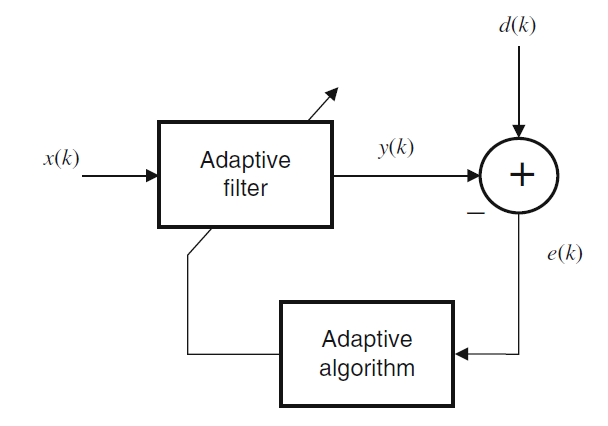
\includegraphics[width=0.9\textwidth]{fA.png}
	\caption{Diagrama de blocos de um filtro adaptativo}
	\label{fig:filtroAdaptativo}
\end{figure}

\indent Filtros adaptativos são considerados sistemas não lineares, portanto a análise de seu comportamento é mais complexa que de a filtros com coeficientes fixos. Por outro lado, pelo fato de serem auto-projetados, por um ponto de vista mais prático, eles podem ser considerados menos complicados que os convencionais em termos de projeto[6].

\indent O desenho usual de um filtro adaptativo pode ser visto na figura \ref{fig:filtroAdaptativo}, onde $k$ é o número da iteração, $x(k)$ é a entrada do filtro, $y(k)$ é o sinal de saída, $d(k)$ é o valor de referência e $e(k)=d(k)-y(k)$ é o valor de erro, necessário para o algoritmo de adaptação do filtro. O algoritmo de adaptação é o prcesso usado para ajustar os coeficientes do filtro de modo a minimizar o erro de acordo com os critétios preestabelecidos. A escolha do algoritmo determina muitos aspectos do processo de adaptação, como a existência de soluções subótimas e complexidade computacional.

\subsection{Adaptação via gradiente descendente}

Uma das formas mais antigas e consagradas de otimizar uma função dentro dos métodos clássicos é seguir a direção do gradiente desta função, com relação as variáveis de interesse, para atualizar os valores destas variáveis de forma iterativa.

Seja um sistema descrito pela série temporal $u[n] \; n=0,1,2..$ e um filtro de resposta impulsiva real $w_0, w_1 ... w_{M-1}$:
\begin{equation}
y[n]=\sum_{k=0}^{M-1}u[n-k]w_k
\end{equation}
Todo este desenvolvimento pode ser feito de maneira bastante similar considerando entradas complexas e filtros com coeficientes complexos, mas por questões de simplicidade será focado o caso em que ambos são reais.Supondo que se deseja que a saída deste filtro seja uma outra série temporal igualmente real $d[n]$, assim o erro seria:
\begin{equation}
e[n]=d[n]-y[n]    
\end{equation}

Considerando o caso de $u$ estocástico, $e[n]$ é uma variável aleatória. Deseja-se então de minimizar a esperança de $e^2[n]$. Seja a função de custo:
\begin{equation}
J=E[e^2[n]]=E[(d[n]-y[n])^2]   
\end{equation}

Definindo nosso operador gradiente $\nabla_k$:
\begin{equation}
\nabla_k J=-2 E[e[n]u[n-k]]   
\end{equation}

Para encontrar o ótimo com relação a esta função de custo, $\nabla_k J$ deve ser igual a zero para todo $k$, como a esperança do produto de duas variáveis aleatórias é sua correlação, $u[n-k]$ e $e[n]$ devem estar descorrelacionadas para todo $k$. A este resultados chamamos princípio da ortogonalidade. Um corolário deste princípio é que $y$ também deve ser ortogonal, ou descorrelacionada com $e[n]$.

\indent É mais conveniente trabalhar com a notação matricial destes resultados. Ao vetor coluna que contém as variáveis aleatórias $u[n-k]$, de k=0 a K=M-1, se chama $\boldsymbol{u}_n$ o vetor de coeficientes $w$, igualmente:

\begin{equation*}
\boldsymbol{u}_n=
\begin{bmatrix}
u[n] & u[n-1] & \dots & u[n-M+1]
\end{bmatrix}^T
\end{equation*}
\begin{equation*}
\boldsymbol{W}_n=
\begin{bmatrix}
w_0 & w_1 & \dots & w_{M-1}
\end{bmatrix}^T
\end{equation*}
Desenvolvendo a equação anterior, obtém-se:

\begin{equation}
\nabla J=-2 E[e[n]\boldsymbol{u}_n]=2E[\boldsymbol{u}_n\boldsymbol{U}^{T}_n\boldsymbol{W}-d[n]\boldsymbol{u}_n]   
\end{equation}

Desta última equação $E[d[n]\boldsymbol{U}_n]$ é o vetor de correlação cruzada entre $d[n]$, ao qual se chama $\boldsymbol{r_{du}}$ e as amostras atrasadas do sinal de entrada. Destacamos também que $E[\boldsymbol{U}_n\boldsymbol{U}^{T}_n]$, a qual chamaremos $\boldsymbol{R_{uu}}$, é a matriz MxM de autocorrelação do mesmo sinal. Sendo assim:

\begin{equation}
\boldsymbol{R}_{uu}\boldsymbol{w}-\boldsymbol{r}_{du}=0
\end{equation}

De onde se conclui que o vetor coeficientes ótimos $\boldsymbol{w}_{opt}$ é:

\begin{equation}
\boldsymbol{w}_{opt}=\boldsymbol{R}_{uu}^{-1}\boldsymbol{r}_{du}
\end{equation}

Se $u$ é um processo estacionário em sentido amplo, então é possível coletar amostras suficientes para fazer uma boa estimação das matrizes acima, encontrando assim um filtro muito mais apropriado para os propósitos deste trabalho. Desta maneira, se estima o conteúdo espectral de $u$ com precisão. Reparemos que este método não é propriamente um gradiente descendente já que encontramos a solução em um passo apenas.

\indent A solução acima tem sua utilidade, entretanto, se a natureza do sinal mudar, não teremos mais uma boa aproximação do mesmo, neste caso, é melhor resolver estas equações de forma recursiva, de modo que o filtro possa se adaptar constantemente à mudanças ocorridas.  

\subsection{O algoritmo LMS}

Para atualizar o vetor de pesos $\boldsymbol{w}_n$ na direção oposta a do gradiente, definimos um coeficiente de aprendizagem $\mu$. A cada iteração vamos fazer o seguinte:

\begin{equation*}
\boldsymbol{w}_{n}=\boldsymbol{w}_{n-1} - \mu \nabla J
\end{equation*}
\begin{equation}
\boldsymbol{w}_{n}=\boldsymbol{w}_{n-1} + \mu(\boldsymbol{r}_{du}-\boldsymbol{R}_{uu} \boldsymbol{w}_{n+1})
\label{eq:w_lms}
\end{equation}

O que diferencia o LMS de outros métodos de gradiente descendente é a forma de estimar as matrizes $\boldsymbol{R}_{uu}$ e $\boldsymbol{r}_{du}$. Estas serão estimadas da seguinte forma:

\begin{equation}
\boldsymbol{\hat{R}}_{uu}=\boldsymbol{u}_n \boldsymbol{u}_{n}^T
\end{equation}
\begin{equation}
\boldsymbol{\hat{r}}_{du}=\boldsymbol{u}_n d[n]
\end{equation}

O que pode soar uma heresia, mas faz sentido se lembra que apenas temos M amostras de sinal.

\subsection{O algoritmo NLMS}

Uma melhoria no algoritmo anterior pode ser proposta. Multiplicando a parte que está entre parênteses na equação \ref{eq:w_lms}:

\begin{equation}
\boldsymbol{w}_{n}=\boldsymbol{w}_{n-1} + \mu \boldsymbol{R}_{uu}^{-1}(\boldsymbol{r}_{du}-\boldsymbol{R}_{uu} \boldsymbol{w}_{n+1}) = \boldsymbol{w}_{n-1} + \mu(\boldsymbol{w}_{opt} - I \boldsymbol{w}_{n-1}) = \boldsymbol{w}_{opt}
\end{equation}

Em teoria, este algoritmo convergiria em apenas uma iteração. Resta o empecilho de estimar tal matriz. Com estimador anterior isto não é possível, porque a matriz estimada $\boldsymbol{\hat{R}}_{uu}$ não é inversível por ser o produto de dois vetores. Mas podemos fazer uma aproximação da forma $\boldsymbol{\hat{R}}_{uu} + \boldsymbol{I} \epsilon$. Que certamente é inversível e confere uma inversa útil, para valores pequenos de $\epsilon$. E após alguma álgebra \cite{bessegato2012line}, que pode ser encontrada em \cite{haykin2005adaptive}, chegamos ao seguinte:

\begin{equation}
\boldsymbol{w}_{n}=\boldsymbol{w}_{n-1} + \mu \frac{\boldsymbol{u}_{n}}{|\boldsymbol{u}_{n}|^2 + \epsilon }(d[n]-\boldsymbol{u}_{n} \boldsymbol{w}_{n-1}) =\boldsymbol{w}_{n-1} + \mu \frac{\boldsymbol{u}_{n}}{|\boldsymbol{u}_{n}|^2 + \epsilon }e[n]
\end{equation}

A este algoritmo se chama LMS normalizado, ou NLMS. Há ainda o estudo de convergência para valores pequenos de $\mu$, que também pode ser encontrado em \cite{diniz1997adaptive} e \cite{haykin2005adaptive}, tanto para o LMS quanto para o NLMS. Mas de modo geral o NLMS deve convergir respeitadas todas as condições estabelecidas anteriormente e escolhendo valores de $\mu<1$.

\subsection{RLS}

\indent O método RLS (\textit{Recursive Least Squares}), ou mínimos quadrados recursivo, é um método de adaptação que visa a minimização da soma dos quadrados da diferença entre o sinal de referência e o sinal de saída do filtro em questão (o erro), assim como os anteriormente mencionados. O RLS pode ser obtido a partir do LMS (\textit{Least Mean Squares}), e é conhecido por possuir rápida convergência, tendo boa performance em sistemas variantes no tempo, como o caso de nosso interesse. Isto vem ao custo de certa complexidade computacional aliada a problemas de estabilidade \cite{diniz1997adaptive}.

\indent Voltando ao modelo do filtro adaptativo da seção anterior, havia sido feita uma estimação bastante simplória de $\boldsymbol{R}_{uu}$ para o LMS, e um pouco mais desenvolvida no NLMS, agora se pode imaginar uma outra: nos casos anteriores somente se aproveitava as M últimas amostras de nosso sinal para cada iteração, mas se por exemplo faz-se uma média das $\boldsymbol{R}_{uu}^{(k)}$ nos aproximamos mais da matriz verdadeira de autocorrelação. Podemos escolher então um novo estimador para $\boldsymbol{R}_{uu}$:

\begin{equation}
\boldsymbol{S}_{d}^{-1}=\boldsymbol{\hat{R}}_{uu}=\frac{1}{k+1}\sum_{i=0}^{k}\lambda^{k-i}\boldsymbol{U}_i\boldsymbol{U}_i^*
\end{equation}

\indent Esta definição em realidade é uma média ponderada em uma série geométrica, e se $\lambda<1$ as últimas amostras contam mais que as primeiras. Reparemos que se $\lambda=1$ tem-se um estimador consistente da matriz. À $\lambda$ se chama fator de esquecimento.


\indent Outra forma de se chegar ao RLS é por sua função objetivo dada por:

\begin{equation}
\xi(k)=\sum_{i=0}^{k}\lambda^{k-i}\varepsilon^2(i)
=\sum_{i=0}^{k}\lambda^{k-i}[d(i)-\boldsymbol{x}(k) \boldsymbol{w}(k)]
\end{equation}

\indent Onde $\varepsilon$ é o erro a posteriori no instante $i$. É possível estimar a matriz $\boldsymbol{R}_{uu}$ de forma recursiva, para evitar cálculos desnecessários, e melhor que isso, sua inversa também pode ser calculada de maneira recursiva, o que é mais importante para nós. A inversa pode ser substituída na expressão obtida para o NLMS. A dedução no entanto não nos interessa tanto no trabalho, ela pode ser encontrada em \cite{haykin2005adaptive} e \cite{diniz1997adaptive}. Ficamos com o resultado final:

\Large
\begin{equation}
\boldsymbol{\phi}^{-1}_k=\lambda^{-1}\Bigg[\boldsymbol{\phi}_{k-1}-\frac{\boldsymbol{\phi}_{k-1}\boldsymbol{u}^T_k\boldsymbol{u}_k\boldsymbol{\phi}_{k-1}}{\lambda+\boldsymbol{u}_k\boldsymbol{\phi}_{k-1}\boldsymbol{u}^T_k}\Bigg]
\end{equation}
\normalsize

\indent Os pesos então podem ser atualizados da seguinte maneira:

\begin{equation}
\boldsymbol{w}_{n}=\boldsymbol{w}_{n-1} +  \boldsymbol{\phi}_{n}^{-1}e[n] \boldsymbol{u}_{n}
\end{equation}

\indent Uma recomendação de inicialização de $\boldsymbol{\phi}_0$ é $\boldsymbol{\phi}_0=\delta \boldsymbol{I}$, sendo $\delta$ o inverso da potência estimada do sinal.



%% ============== PLL ========================



\section{PLL}

\indent Um Phase Locked Loop digital, assim como sua versão analógica, visa determinar os parâmetros de um processo estocástico como uma onda senoidal. Desta forma o PLL tenta estimar parâmetros de Amplitude, fase e frequência. Temos diversas variantes digitais e analógicas \cite{al2006digital}, a variante utilizada neste trabalho foi proposta por Ziarani em 2004 \cite{ziarani2004method}. Uma breve demostração será realizada abaixo.
\indent Seja $u(t)$ uma função variante no tempo, e $y(t)=Asin\phi(t)$ um sinal periódico senoidal sendo $A$ a amplitude do sinal e $\phi(t)$ sua fase, tendo este sinal uma frequência constante, podemos escrever $\phi(t)=wt+\delta$, sendo $w$ igual a frequência e $\delta$ um valor de fase constante. Escrevendo de maneira mais geral:

\begin{equation}
u(t)=\sum_{i=0}^{\infty}A_i sin\phi_i(t)\space+\space n(t)
\end{equation}

Onde $n(t)$ representa um distúrbio, como um ruído. Na realidade, todos os parâmetros podem variar com o tempo, é conveniente escrever então um conjunto $\Psi(t)=[A(t), w(t), \delta(t)]$ o qual contém todos os parâmetros de um possível sinal $y(t)$.

Definimos a função $d$:
\begin{equation}
d^2(t,\Psi(t))=[u(t)-y(t,\Psi(t))]^2=e^2(t)
\end{equation}

Assim sendo o conjunto $\Psi(t)$ ótimo o que minimiza a função $d^2$ que será adotado como função de custo $J(\Psi(t),t)$. Os parâmetros $\Psi(t)$ podem ser estimados por meio de gradiente descendente.

\begin{equation}
\frac{d\Psi(t)}{dt}=-\boldsymbol{\mu}\frac{\partial J(\Psi(t),t)}{\partial \Psi(t)}
\
\end{equation}

\begin{equation}
\boldsymbol{\mu}=
\begin{bmatrix}
m_1 && 0 && 0 \\
0 && m_2 && 0 \\
0 && 0 && m_3
\end{bmatrix}
\end{equation}

Com $\frac{d\Psi(t)}{dt}$ denotando o vetor na direção do qual são atualizados os valores de $\Psi(t)$ a cada iteração. E $\boldsymbol{\mu}$ a matriz diagonal contendo as constantes de atualização referentes a cada parâmetro. Como estaremos lidando com estimações agora, usaremos a notação $\hat{\Psi}(t)$:

\begin{equation}
\begin{bmatrix}
\frac{d\hat{A}(t)}{dt} \\
\frac{d\hat{w}(t)}{dt}\\
\frac{d\hat{\delta}(t)}{dt}
\end{bmatrix}
=-\boldsymbol{\mu}
\begin{bmatrix}
\frac{\partial e^2(t)}{\partial \hat{A}} \\
\frac{\partial e^2(t)}{\partial \hat{w}} \\
\frac{\partial e^2(t)}{\partial \hat{\delta}}
\end{bmatrix}
\end{equation}

Obtém-se então o seguinte:
\begin{equation}
\frac{d\hat{A}(t)}{dt}=2m_1e(t)sin(\int_{0}^{t}\hat{w}(\tau)d\tau\space+\space\hat{\delta}(t))
\end{equation}
\begin{equation}
\frac{d\hat{w}(t)}{dt}=2m_2e(t)\hat{A}(t)tcos(\int_{0}^{t}\hat{w}(\tau)d\tau\space+\space\hat{\delta}(t))
\end{equation}
\begin{equation}
\frac{d\hat{\delta}(t)}{dt}=2m_3e(t)\hat{A}(t)cos(\int_{0}^{t}\hat{w}(\tau)d\tau\space+\space\hat{\delta}(t))
\end{equation}
\begin{equation}
\frac{d\hat{\phi}(t)}{dt}=\hat{w}(t)+\frac{\hat{\delta}(t)}{dt}
\end{equation}

Por conta do fator temporal $t$ que aparece solto na equação referente a $\hat{w}$, esse sistema é variante no tempo, o que o torna instável. No entanto uma solução heurística é substituir $t$ por uma constante $m4$, que pode ser absorvida pela constante $m2$, tornando o sistema invariante no tempo e fazendo com que este sistema de equações seja útil na prática. Desta maneira tem-se o seguinte:
\begin{equation}
\frac{d\hat{A}(t)}{dt}=2\mu_1e(t)sin(\int_{0}^{t}\hat{w}(\tau)d\tau\space+\space\hat{\delta}(t))
\end{equation}
\begin{equation}
\frac{d\hat{w}(t)}{dt}=2\mu_2e(t)\hat{A}(t)tcos(\int_{0}^{t}\hat{w}(\tau)d\tau\space+\space\hat{\delta}(t))
\end{equation}
\begin{equation}
\frac{d\hat{\phi}(t)}{dt}=\hat{w}(t)+2\mu_3e(t)\hat{A}(t)cos(\int_{0}^{t}\hat{w}(\tau)d\tau\space+\space\hat{\delta}(t))
\end{equation}

Usando o método \textit{Euler Forward}:

\begin{equation}
A[n+1]=A[n]+\mu_1T_s e[n]sen(\phi(t))
\end{equation}
\begin{equation}
w[n+1]=w[n]+\mu_2T_s e[n]cos(\phi(t))
\end{equation}
\begin{equation}
\phi[n+1]=\phi[n] + T_s w[n] + \mu_3T_s e[n]cos(\phi(t))
\end{equation}

Está definido o conjunto de equações discretas que serão utilizadas para rastrear frequências no restante do trabalho.

\begin{figure}[h]
	\centering    
	\def\svgwidth{\columnwidth}
	\input{images/pll_basico.pdf_tex}
	\caption{Convergência do PLL com a presença de apenas a fundamental}
	\label{fig:your image label}
\end{figure}

%=============Multitaxa================

\section{Processamento Multitaxa}

Em determinadas situações, é desejável alterar a taxa de amostragem de um sinal para realizar certos tipos de processamento. Por exemplo, veremos em alguns resultados nas próximas sessões que o algoritmo PLL descrito anteriormente é sensível a taxa de amostragem em relação a frequência rastreada, portanto é conveniente mantê-la mais ou menos constante. Também veremos que processar sinais na taxa necessária para abranger todo o espectro que se quer analisar é extremamente custoso computacionalmente e não é garantia de melhores resultados. Por isso deve-se considerar o uso de uma estrutura multitaxa que diminua a frequência base.

\indent Serão analisadas a seguir as implicações de um abaixamento na frequência de amostragem:

\subsection{Downsampling}

Uma estrutura downsampling tem a forma seguinte:

\tikzstyle{int}=[draw, fill=blue!20, minimum size=2em]
\tikzstyle{init} = [pin edge={to-,thin,black}]

\begin{center}
	\begin{tikzpicture}[node distance=2.5cm,auto,>=latex']
	\node [int] (a) {$M_k \downarrow$};
	\node (b) [left of=a,node distance=2cm, coordinate] {a};
	%\node [int, pin={[init]above:$p_0$}] (c) [right of=a] {$\frac{1}{s}$};
	\node [coordinate] (end) [right of=b, node distance=4cm]{};
	\path[->] (b) edge node {$x(k)$} (a);
	\draw[->] (a) edge node {$y(k)$} (end) ;
	\end{tikzpicture}
\end{center}


Representamos a estrutura como um sistema que reproduz em sua saída apenas amostras onde $k$ é múltiplo de $M_k$. Podemos escrever $y[n]=x[nM_k] \; n=1,2,3...$ Considerando que $x[k]$ foi amostrado com a frequência de Nyquist $fs$, o efeito final é o mesmo que se tivéssemos amostrado $x$ com $fs/M_k$, podemos dizer que vamos observar aliasing em nosso resultado final. Haverá portanto sobreposição no espectro de frequência referente a $X(w)$ quando analisarmos $Y(w)$. Entretanto, é possível prever onde estarão localizadas as componentes espectrais presentes no sinal completo que estamos subamostrando, e embora não possamos saber exatamente qual é o valor correspondente as frequências originais, podemos saber no mínimo qual é sua soma.

\indent Uma demonstração formal dos efeitos observados pode ser encontrada em \cite{mitra2006digital}, aqui faremos uma abordagem mais intuitiva. Dada uma componente espectral de $x[k]$ referente a $w_0$. Supõe-se que é feita uma subamostragem neste sinal, e agora sua frequência de amostragem que era $f_s$ se torna $f_s/M_k$. Agora, se $w_0<f_s/(2Mk)$ essa as componentes dessa frequência não saem do lugar, elas continuam onde estavam anteriormente. Isso não significa que seu espectro não seja alterado nas frequências mais baixas que a nova taxa de amostragem, somente quer dizer que elas sofrem interferência no mesmo lugar onde estavam antes. Agora, se a frequência de interesse é maior que a nova frequência de amostragem dividida por 2, então ela não poderá de forma alguma ser encontrada no mesmo local, pois simplesmente não há como visualizá-la com DFT ou DTFT. Mas então onde vão parar essas frequências? Bom, onde pararia qualquer uma que sofre aliasing. Ela dá voltas no círculo de frequências. O circulo de frequências sempre vai de 0 a $2\pi$, e as frequências sempre caminham nele no sentido anti-horário. Para cada vez que a frequência de interesse (a qual chamaremos $f_i$) for maior que $fs$, a frequência em questão dá uma volta no círculo. Um algoritmo simples será apresentado quando expusermos o método do PLL multitaxa, mas por hora podemos saber que o ângulo referente à nova frequência será o resto da divisão $f_i/f_s$ e multiplicamos por $2\pi$. 

\begin{figure}[H]
	\centering
	\def\svgwidth{\columnwidth}
	\input{images/no_aliasing.pdf_tex}
	\caption{Downsampling para $f_s=160Hz$, $f_0=10Hz$, $M_k=5$}
	\label{fig:no_aliasing}
\end{figure}

No exemplo da figura \ref{fig:no_aliasing}, temos $fs=160Hz$ e $M_k=5$, a frequência de interesse é 10Hz, a frequência de amostragem depois da subamostragem seria ainda maior que $2f_i$, então ela não se move, como observado na figura. Entretanto, no caso de $M_k=10$ a coisa muda, calculando:

\begin{equation}
w_i=rest(f_i \: M_k, \: f_s)2\pi
\end{equation}

\begin{figure}[H]
	\centering
	\def\svgwidth{\columnwidth}
	\input{images/aliasing.pdf_tex}
	\caption{Downsampling para $f_s=160Hz$, $f_0=10Hz$, $M_k=10$}
	\label{fig:aliasing}
\end{figure}

Como resultado tem-se $\frac{5}{4}\pi$ que é maior que é ligeiramente maior que $\pi$ portanto já se pode saber que esta componente sofre aliasing, como se nota na figura \ref{fig:aliasing}.